\documentclass[12pt,a4paper]{article}

% ─── Paquetes ────────────────────────────────────────────────────────────────
\usepackage[utf8]{inputenc}
\usepackage[T1]{fontenc}
\usepackage[spanish,es-nodecimaldot]{babel}
\usepackage{lmodern}
\usepackage{geometry}
\usepackage{graphicx}
\usepackage{booktabs}
\usepackage{longtable}
\usepackage{array}
\usepackage{tabularx}
\usepackage{multirow}
\usepackage{amsmath}
\usepackage{amssymb}
\usepackage{hyperref}
\usepackage{xcolor}
\usepackage{listings}
\usepackage{caption}
\usepackage{subcaption}
\usepackage{float}
\usepackage{fancyhdr}
\usepackage{titlesec}
\usepackage{setspace}
\usepackage{parskip}
\usepackage{enumitem}
\usepackage{mdframed}
\usepackage{tcolorbox}
\usepackage{tikz}
\usepackage{pgfplots}
\pgfplotsset{compat=1.18}

% ─── Geometría ───────────────────────────────────────────────────────────────
\geometry{
  top=2.5cm, bottom=2.5cm,
  left=3cm, right=2.5cm,
  headheight=15pt
}

% ─── Colores institucionales ─────────────────────────────────────────────────
\definecolor{azulUDG}{RGB}{0, 60, 130}
\definecolor{grisFondo}{RGB}{245, 247, 250}
\definecolor{verdeMetrica}{RGB}{34, 139, 34}
\definecolor{rojoAlerta}{RGB}{180, 30, 30}
\definecolor{grisTexto}{RGB}{80, 80, 80}

% ─── Encabezados y pies de página ────────────────────────────────────────────
\pagestyle{fancy}
\fancyhf{}
\fancyhead[L]{\small\textcolor{azulUDG}{\textit{Diagnóstico Predictivo de Diabetes — UDG}}}
\fancyhead[R]{\small\textcolor{grisTexto}{\thepage}}
\fancyfoot[C]{\small\textcolor{grisTexto}{Materia: Procesamiento de Datos / Inteligencia Artificial}}
\renewcommand{\headrulewidth}{0.4pt}
\renewcommand{\footrulewidth}{0.2pt}

% ─── Estilo de secciones ─────────────────────────────────────────────────────
\titleformat{\section}[block]
  {\large\bfseries\color{azulUDG}}
  {\thesection.}{0.5em}{}[\titlerule]
\titleformat{\subsection}[block]
  {\normalsize\bfseries\color{azulUDG!80!black}}
  {\thesubsection.}{0.5em}{}
\titleformat{\subsubsection}[runin]
  {\normalsize\bfseries\color{grisTexto}}
  {\thesubsubsection.}{0.4em}{}[.\quad]

% ─── Cajas informativas ──────────────────────────────────────────────────────
\tcbuselibrary{skins,breakable}
\newtcolorbox{infobox}[1][]{
  colback=grisFondo, colframe=azulUDG,
  fonttitle=\bfseries\small, title={#1},
  boxrule=0.5pt, arc=3pt,
  breakable
}
\newtcolorbox{alertbox}[1][Nota clínica]{
  colback=red!5, colframe=rojoAlerta,
  fonttitle=\bfseries\small\color{rojoAlerta}, title={#1},
  boxrule=0.5pt, arc=3pt
}

% ─── Código fuente ───────────────────────────────────────────────────────────
\lstset{
  basicstyle=\ttfamily\small,
  backgroundcolor=\color{grisFondo},
  frame=single, framerule=0.4pt, frameround=tttt,
  breaklines=true, breakatwhitespace=true,
  columns=fullflexible, keepspaces=true,
  numbers=left, numberstyle=\tiny\color{grisTexto},
  language=Python,
  keywordstyle=\color{azulUDG}\bfseries,
  stringstyle=\color{verdeMetrica},
  commentstyle=\color{grisTexto}\itshape,
}

% ─── Metadatos ───────────────────────────────────────────────────────────────
\hypersetup{
  pdftitle={Reporte Técnico-Académico: Diagnóstico Predictivo de Diabetes},
  pdfauthor={CCMarv},
  pdfsubject={Procesamiento de Datos / Inteligencia Artificial},
  colorlinks=true, linkcolor=azulUDG, urlcolor=azulUDG!70!black,
  citecolor=azulUDG
}

% ─── Interlineado ────────────────────────────────────────────────────────────
\setstretch{1.15}

% ═══════════════════════════════════════════════════════════════════════════════
\begin{document}

% ─── PORTADA ────────────────────────────────────────────────────────────────
\begin{titlepage}
  \centering
  \vspace*{1cm}

  {\color{azulUDG}\rule{\linewidth}{1.5pt}}
  \vspace{0.3cm}

  {\LARGE\bfseries\color{azulUDG}
    Reporte Técnico-Académico\\[0.4em]
    \large Sistema de Diagnóstico Predictivo de Diabetes\\[0.2em]
    \normalsize mediante Aprendizaje Supervisado y No Supervisado
  }

  \vspace{0.3cm}
  {\color{azulUDG}\rule{\linewidth}{1.5pt}}
  \vspace{1cm}

  \begin{tabular}{ll}
    \textbf{Repositorio:}    & \texttt{CCMarv/Diasgnostico-pred}\\[4pt]
    \textbf{Asignatura:}     & Procesamiento de Datos / Inteligencia Artificial\\[4pt]
    \textbf{Institución:}    & Universidad de Guadalajara (UDG)\\[4pt]
    \textbf{Dataset base:}   & CDC BRFSS 2015 — 253{,}680 registros\\[4pt]
    \textbf{Fecha:}          & 2026-05-18\\[4pt]
    \textbf{Semilla global:} & 42 (reproducible)\\
  \end{tabular}

  \vspace{1.5cm}

  \begin{infobox}[Corridas de referencia utilizadas en este reporte]
    \begin{tabular}{lllll}
      \toprule
      \textbf{Corrida} & \textbf{Muestras} & \textbf{Mejor modelo} & \textbf{ROC-AUC} & \textbf{Tiempo}\\
      \midrule
      10k & 10{,}000 & SVM & 0.8351 & 111 s\\
      50k & 50{,}000 & GBM & 0.8270 & 2{,}939 s\\
      \bottomrule
    \end{tabular}
  \end{infobox}

  \vfill

  {\small\color{grisTexto}
    Artefactos de trazabilidad: \texttt{report-output/evidence.log},
    \texttt{report-output/metrics.csv}\\
    Código fuente: \url{https://github.com/CCMarv/Diasgnostico-pred}
  }
\end{titlepage}

% ─── TABLA DE CONTENIDOS ─────────────────────────────────────────────────────
\tableofcontents
\newpage

% ═══════════════════════════════════════════════════════════════════════════════
\section{Resumen ejecutivo}

Este reporte documenta el diseño, implementación y evaluación de un sistema de estimación de riesgo de diabetes tipo 2 basado en técnicas de aprendizaje automático. El proyecto utiliza datos del \textit{Behavioral Risk Factor Surveillance System} (BRFSS) 2015 del CDC de los Estados Unidos y abarca un flujo completo de procesamiento de datos: desde la carga y limpieza del dataset hasta el despliegue en API REST y dashboard interactivo.

Se compararon cuatro modelos supervisados —\textbf{SVM}, \textbf{Árbol de Decisión}, \textbf{GBM} y \textbf{MLP}— bajo un protocolo experimental uniforme con validación cruzada estratificada, preprocesamiento encapsulado en pipeline serializable y manejo de desbalance de clases mediante SMOTE. Adicionalmente, se implementó \textbf{K-Means} para identificar fenotipos de riesgo clínico de forma no supervisada.

Los resultados más relevantes son:

\begin{itemize}[noitemsep]
  \item Con $n=10{,}000$: \textbf{SVM} obtuvo el mejor ROC-AUC ($0.8351$) con sensibilidad de $77.2\%$.
  \item Con $n=50{,}000$: \textbf{GBM} obtuvo el mejor ROC-AUC ($0.8270$) con especificidad de $92.9\%$.
  \item K-Means identificó dos fenotipos con diferencia de prevalencia de \textbf{15.1 pp} ($p{<}0.001$).
  \item El pipeline cumple con los modelos del temario: SVM, Árbol, MLP, GBM, K-Means.
\end{itemize}

\begin{alertbox}[Limitación principal]
  El dataset proviene de población estadounidense. Se documentan sesgos distribucionales significativos respecto a México (ENSANUT 2022) en 6 de 10 variables clave, lo que impide la transferencia directa del modelo sin ajuste de calibración o reentrenamiento.
\end{alertbox}

% ═══════════════════════════════════════════════════════════════════════════════
\section{Introducción y contexto epidemiológico}

\subsection{Problema de salud pública}

La diabetes mellitus tipo 2 es una de las enfermedades crónico-degenerativas con mayor carga epidemiológica en México y en el mundo. Según datos de la Encuesta Nacional de Salud y Nutrición (ENSANUT 2022), la prevalencia en adultos mexicanos mayores de 20 años supera el $12\%$, con una tendencia ascendente asociada al envejecimiento poblacional, el cambio en los patrones de alimentación y la reducción de la actividad física. De manera preocupante, se estima que hasta el $40\%$ de los casos en México no han recibido diagnóstico formal al momento en que ocurre su primer evento clínico severo.

El diagnóstico tardío genera una cadena de consecuencias: tratamiento más costoso, mayor riesgo de complicaciones (nefropatía, retinopatía, neuropatía, pie diabético), mayor mortalidad cardiovascular y saturación de servicios de segundo y tercer nivel de atención. En este contexto, los sistemas de tamizaje predictivo representan una herramienta de salud pública de primer nivel: al ordenar a la población por nivel de riesgo estimado, permiten focalizar los recursos de detección hacia los grupos con mayor probabilidad de diagnóstico positivo, sin necesidad de pruebas de laboratorio costosas.

\subsection{Justificación del enfoque computacional}

Los modelos de aprendizaje automático son particularmente adecuados para tareas de tamizaje cuando se dispone de variables de fácil recolección (cuestionarios de conducta y salud autorreportada) y cuando la población objetivo es heterogénea. A diferencia de los modelos de regresión logística tradicionales, los algoritmos de \textit{machine learning} pueden capturar interacciones no lineales entre variables (e.g., la combinación de obesidad, hipertensión y edad avanzada tiene un efecto multiplicativo, no aditivo, sobre el riesgo de diabetes).

Este proyecto demuestra que es posible construir un clasificador con ROC-AUC $\approx 0.83$ usando exclusivamente las 21 variables de conducta del BRFSS, sin acceso a datos de laboratorio. Esto posiciona al sistema como una herramienta viable para tamizaje de \textbf{primer nivel} en unidades de medicina familiar.

\subsection{Dataset: CDC BRFSS 2015}

El \textbf{Behavioral Risk Factor Surveillance System (BRFSS)} es la encuesta de salud telefónica más grande del mundo, aplicada anualmente a adultos estadounidenses por los Centros para el Control y la Prevención de Enfermedades (CDC). La versión 2015 contiene $253{,}680$ registros con información completa o parcialmente imputada.

\begin{table}[H]
  \centering
  \caption{Estructura del dataset CDC BRFSS 2015}
  \label{tab:dataset}
  \begin{tabular}{lll}
    \toprule
    \textbf{Atributo} & \textbf{Valor} & \textbf{Observación}\\
    \midrule
    Registros totales & 253{,}680 & Adultos EE.UU. 2015\\
    Variables predictoras & 21 & Conducta, salud, sociodemografía\\
    Variable objetivo & \texttt{Diabetes\_binary} & 0=sin diabetes, 1=con diabetes/prediabetes\\
    Desbalance de clases & 6.2:1 & 86.2\% clase 0, 13.8\% clase 1\\
    Valores faltantes & Parciales & Presentes en \texttt{BMI}, \texttt{MentHlth}, \texttt{PhysHlth}\\
    \bottomrule
  \end{tabular}
\end{table}

\begin{table}[H]
  \centering
  \caption{Variables predictoras del dataset (21 columnas CDC)}
  \label{tab:variables}
  \small
  \begin{tabularx}{\linewidth}{llXl}
    \toprule
    \textbf{Variable} & \textbf{Tipo} & \textbf{Descripción} & \textbf{Rango}\\
    \midrule
    \texttt{HighBP} & Binaria & Diagnóstico previo de hipertensión arterial & 0–1\\
    \texttt{HighChol} & Binaria & Diagnóstico previo de colesterol alto & 0–1\\
    \texttt{CholCheck} & Binaria & Prueba de colesterol en últimos 5 años & 0–1\\
    \texttt{BMI} & Continua & Índice de masa corporal (kg/m²) & 10–80\\
    \texttt{Smoker} & Binaria & $\geq$100 cigarrillos en su vida & 0–1\\
    \texttt{Stroke} & Binaria & Derrame cerebral previo & 0–1\\
    \texttt{HeartDiseaseorAttack} & Binaria & Cardiopatía o infarto previo & 0–1\\
    \texttt{PhysActivity} & Binaria & Actividad física en últimos 30 días & 0–1\\
    \texttt{Fruits} & Binaria & Fruta $\geq$1 vez al día & 0–1\\
    \texttt{Veggies} & Binaria & Verdura $\geq$1 vez al día & 0–1\\
    \texttt{HvyAlcoholConsump} & Binaria & Consumo elevado de alcohol & 0–1\\
    \texttt{AnyHealthcare} & Binaria & Algún tipo de cobertura médica & 0–1\\
    \texttt{NoDocbcCost} & Binaria & Evitó médico por costo & 0–1\\
    \texttt{GenHlth} & Ordinal & Salud autorreportada (1=excelente, 5=mala) & 1–5\\
    \texttt{MentHlth} & Continua & Días de mala salud mental (último mes) & 0–30\\
    \texttt{PhysHlth} & Continua & Días de mala salud física (último mes) & 0–30\\
    \texttt{DiffWalk} & Binaria & Dificultad para caminar o subir escaleras & 0–1\\
    \texttt{Sex} & Binaria & 0=Femenino, 1=Masculino & 0–1\\
    \texttt{Age} & Ordinal & Grupo etario CDC (1=18–24, 13=$\geq$80) & 1–13\\
    \texttt{Education} & Ordinal & Nivel educativo (1=sin escolaridad, 6=universitario+) & 1–6\\
    \texttt{Income} & Ordinal & Ingreso relativo (1=$<$\$10k, 8=$>$\$75k) & 1–8\\
    \bottomrule
  \end{tabularx}
\end{table}

% ═══════════════════════════════════════════════════════════════════════════════
\section{Análisis exploratorio de datos (EDA)}

\subsection{Distribución y calidad de los datos}

El análisis exploratorio del dataset reveló cuatro características estructurales que condicionaron todas las decisiones de preprocesamiento posteriores:

\begin{enumerate}
  \item \textbf{Desbalance severo de clases:} La prevalencia de diabetes en el dataset es del $13.8\%$ ($n=35{,}017$ casos positivos de 253{,}680 totales), lo que resulta en un ratio de desbalance de $6.2:1$. Un clasificador que siempre predijera la clase mayoritaria obtendría una \textit{accuracy} del $86.2\%$, lo que ilustra por qué la accuracy no es una métrica apropiada para este problema. La decisión de usar ROC-AUC como métrica primaria es directamente consecuencia de este desbalance.

  \item \textbf{Variables continuas con distribución asimétrica:} \texttt{BMI}, \texttt{MentHlth} y \texttt{PhysHlth} presentan distribuciones marcadamente asimétricas a la derecha, con valores extremos que distorsionarían la imputación por mediana simple. El BMI tiene una distribución aproximadamente bimodal con moda principal alrededor de $25$--$27$ kg/m² y una cola larga hacia valores de obesidad severa ($>40$ kg/m²).

  \item \textbf{Variables ordinales con orden clínico real:} \texttt{GenHlth}, \texttt{Age}, \texttt{Education} e \texttt{Income} tienen un orden cardinal clínicamente significativo. Tratarlas como nominales (con \textit{one-hot encoding}) eliminaría información relevante sobre la progresión de riesgo con la edad o el deterioro de la salud general.

  \item \textbf{Correlaciones entre variables de riesgo:} Las variables de comorbilidad (\texttt{HighBP}, \texttt{HighChol}, \texttt{HeartDiseaseorAttack}) presentan correlaciones positivas entre sí y con la variable objetivo, lo que es consistente con la fisiopatología del síndrome metabólico.
\end{enumerate}

\subsection{Contraste distribucional CDC BRFSS 2015 vs.\ ENSANUT 2022}

Una parte central del análisis exploratorio fue la comparación de las distribuciones del dataset con las prevalencias observadas en México según ENSANUT 2022. Este contraste es imprescindible para evaluar la transferibilidad del modelo entrenado.

\begin{table}[H]
  \centering
  \caption{Sesgo distribucional CDC BRFSS 2015 vs.\ México (ENSANUT 2022)}
  \label{tab:sesgo}
  \begin{tabular}{lrrl}
    \toprule
    \textbf{Variable} & \textbf{CDC BRFSS (\%)} & \textbf{ENSANUT 2022 (\%)} & \textbf{Sesgo relativo}\\
    \midrule
    \texttt{Smoker} & 44.5 & 15.8 & \textcolor{rojoAlerta}{$+182\%$ (crítico)}\\
    \texttt{HighChol} & 42.6 & 22.9 & \textcolor{rojoAlerta}{$+86\%$ (alto)}\\
    \texttt{PhysActivity} & 75.6 & 45.2 & \textcolor{rojoAlerta}{$+67\%$ (alto)}\\
    \texttt{Veggies} & 80.9 & 54.8 & $+48\%$ (moderado)\\
    \texttt{HighBP} & 42.8 & 31.8 & $+35\%$ (moderado)\\
    \texttt{AnyHealthcare} & 95.0 & 76.2 & $+25\%$ (moderado)\\
    \texttt{Fruits} & 63.3 & 55.6 & $+14\%$ (bajo)\\
    \texttt{HvyAlcoholConsump} & 5.7 & 5.3 & $+8\%$ (bajo)\\
    \bottomrule
  \end{tabular}
  \smallskip\\
  \footnotesize Fuente: \texttt{notebooks\_processed/01\_eda\_regionalizado\_extract.md}, ENSANUT 2022.
\end{table}

La tabla muestra que $6$ de $8$ variables comparables presentan sesgo moderado o alto, y tres variables (\texttt{Smoker}, \texttt{HighChol}, \texttt{PhysActivity}) tienen diferencias mayores al $50\%$ relativo. Esto implica que el modelo entrenado sobre BRFSS, si se aplicara directamente sobre datos mexicanos, sobreestimaría la prevalencia de tabaquismo y colesterol alto en la población, alterando la distribución de probabilidades predichas. El ajuste del umbral de decisión (de $0.50$ a aproximadamente $0.25$--$0.30$) es la primera medida correctiva recomendada para un despliegue real en contexto IMSS.

% ═══════════════════════════════════════════════════════════════════════════════
\section{Preprocesamiento de datos}

\subsection{Arquitectura del pipeline}

El preprocesamiento está encapsulado en un objeto \texttt{ColumnTransformer} de \texttt{scikit-learn}, que aplica transformaciones diferenciadas según el tipo de variable. El pipeline completo tiene la forma:

\begin{equation}
  \text{Pipeline} = \text{ColumnTransformer} \xrightarrow{\text{SMOTE}} \text{Estimador}
\end{equation}

Esta arquitectura garantiza dos propiedades críticas para la validez experimental:

\begin{enumerate}[noitemsep]
  \item \textbf{Ausencia de data leakage:} todos los parámetros del preprocesador (media, varianza, vecinos KNN, categorías ordinales) se ajustan exclusivamente sobre el conjunto de entrenamiento (\texttt{X\_train}). El conjunto de prueba (\texttt{X\_test}) es transformado, no usado para ajuste.
  \item \textbf{Simetría entrenamiento/inferencia:} al serializar el pipeline completo en un archivo \texttt{.joblib}, la misma transformación se aplica automáticamente en producción (API FastAPI / dashboard Streamlit), garantizando que los datos de un paciente real sean procesados exactamente igual que durante el entrenamiento.
\end{enumerate}

\begin{figure}[H]
  \centering
  \begin{tikzpicture}[
    box/.style={draw=azulUDG, fill=grisFondo, rounded corners=3pt,
                minimum width=3.5cm, minimum height=1cm, align=center,
                font=\small},
    arrow/.style={->, thick, color=azulUDG},
    node distance=1.5cm
  ]
    \node[box] (raw) {Datos crudos\\(253{,}680 × 22)};
    \node[box, below=of raw] (split) {Split 80/20\\estratificado};
    \node[box, below left=1.2cm and 2cm of split] (ct) {ColumnTransformer\\(3 ramas)};
    \node[box, below=of ct] (smote) {SMOTE\\(solo train)};
    \node[box, below=of smote] (model) {Estimador\\(SVM/GBM/MLP/Árbol)};
    \node[box, below right=1.2cm and 2cm of split] (test) {Test set\\(sin tocar)};
    \node[box, below=of model] (eval) {Evaluación\\(métricas clínicas)};

    \draw[arrow] (raw) -- (split);
    \draw[arrow] (split) -- node[left,font=\tiny]{80\%} (ct);
    \draw[arrow] (split) -- node[right,font=\tiny]{20\%} (test);
    \draw[arrow] (ct) -- (smote);
    \draw[arrow] (smote) -- (model);
    \draw[arrow] (model) -- (eval);
    \draw[arrow] (test) -- (eval);
  \end{tikzpicture}
  \caption{Diagrama del pipeline de preprocesamiento y evaluación}
  \label{fig:pipeline}
\end{figure}

\subsection{Ramas del ColumnTransformer}

\subsubsection{Rama 1 — Variables continuas}

Las tres variables continuas (\texttt{BMI}, \texttt{MentHlth}, \texttt{PhysHlth}) son procesadas con dos pasos:

\begin{table}[H]
  \centering
  \caption{Transformaciones para variables continuas}
  \begin{tabular}{lll}
    \toprule
    \textbf{Paso} & \textbf{Clase sklearn} & \textbf{Parámetros}\\
    \midrule
    Imputación & \texttt{KNNImputer} & \texttt{n\_neighbors=5, weights='uniform'}\\
    Escalado & \texttt{StandardScaler} & \texttt{with\_mean=True, with\_std=True}\\
    \bottomrule
  \end{tabular}
\end{table}

La elección de \texttt{KNNImputer} sobre la imputación por mediana se justifica por las distribuciones asimétricas de las tres variables: el BMI puede alcanzar valores de $99$ kg/m² en registros extremos, y reemplazar valores faltantes con la mediana global ($\approx 27$ kg/m²) distorsionaría casos de obesidad severa que son, precisamente, los de mayor riesgo de diabetes. La imputación por $k$ vecinos más cercanos respeta la estructura local de los datos, asignando a cada valor faltante el promedio ponderado de sus $5$ registros más similares en el espacio de las demás variables.

\subsubsection{Rama 2 — Variables binarias}

Las 14 variables binarias (\texttt{HighBP}, \texttt{HighChol}, \texttt{Smoker}, etc.) son procesadas con imputación por moda (\texttt{SimpleImputer(strategy='most\_frequent')}) y conservadas sin escalado (\texttt{passthrough}). La razón de no aplicar \texttt{StandardScaler} a variables binarias es que ya están en la escala óptima: centrarlas en $0.5$ y expandirlas a $\pm 0.5$ no aporta información adicional a los modelos de árbol y penaliza la interpretabilidad de la salida para SVM y MLP.

\subsubsection{Rama 3 — Variables ordinales}

Las cuatro variables ordinales (\texttt{GenHlth}, \texttt{Age}, \texttt{Education}, \texttt{Income}) son codificadas con \texttt{OrdinalEncoder} con rangos predefinidos:

\begin{table}[H]
  \centering
  \caption{Codificación ordinal de variables categóricas con orden clínico}
  \begin{tabular}{llll}
    \toprule
    \textbf{Variable} & \textbf{Rango} & \textbf{Semántica del extremo bajo} & \textbf{Semántica del extremo alto}\\
    \midrule
    \texttt{GenHlth} & 1–5 & Excelente & Mala\\
    \texttt{Age} & 1–13 & 18–24 años & $\geq$80 años\\
    \texttt{Education} & 1–6 & Sin escolaridad & Universitario+\\
    \texttt{Income} & 1–8 & $<$\$10k/año & $>$\$75k/año\\
    \bottomrule
  \end{tabular}
\end{table}

La especificación explícita del rango completo de categorías en el \texttt{OrdinalEncoder} cumple una función doble: preserva el orden clínico real (mayor edad $\rightarrow$ mayor riesgo; mayor ingreso $\rightarrow$ menor riesgo relativo) y previene errores de inferencia cuando valores válidos que no aparecieron en el conjunto de entrenamiento son enviados a la API en producción.

\subsection{Manejo del desbalance de clases — SMOTE}

El desbalance $6.2:1$ en la variable objetivo requiere una estrategia activa. Se aplicó \textbf{SMOTE} (Synthetic Minority Oversampling Technique) mediante \texttt{ImbPipeline} de la librería \texttt{imbalanced-learn}. Los parámetros utilizados fueron:

\begin{table}[H]
  \centering
  \caption{Configuración de SMOTE}
  \begin{tabular}{lll}
    \toprule
    \textbf{Parámetro} & \textbf{Valor} & \textbf{Justificación}\\
    \midrule
    \texttt{k\_neighbors} & 5 (default) & Equilibrio entre localidad y estabilidad\\
    \texttt{random\_state} & \textit{None} & Variación aleatoria en muestras sintéticas\\
    \texttt{sampling\_strategy} & \texttt{'auto'} & Resamplea solo hasta igualar clases\\
    \textbf{Posición en pipeline} & Post-preprocesador, pre-estimador & \textbf{Evita data leakage}\\
    \bottomrule
  \end{tabular}
\end{table}

\begin{alertbox}[Por qué SMOTE debe estar dentro del pipeline, no antes del split]
  Si SMOTE se aplica al dataset completo antes de dividir en train/test, las muestras sintéticas generadas a partir de registros reales de \texttt{X\_test} contaminarían el conjunto de entrenamiento. El modelo ``vería'' versiones artificiales de sus propios datos de prueba, inflando artificialmente todas las métricas de evaluación. Al colocar SMOTE dentro del \texttt{ImbPipeline}, la síntesis de muestras ocurre únicamente sobre \texttt{X\_train}, dentro de cada fold de validación cruzada.
\end{alertbox}

% ═══════════════════════════════════════════════════════════════════════════════
\section{Modelos implementados}

\subsection{Catálogo de modelos}

El proyecto implementa cuatro modelos supervisados y un modelo no supervisado, cubriendo el catálogo del temario de la materia:

\begin{table}[H]
  \centering
  \caption{Modelos implementados y su clasificación en el temario}
  \label{tab:modelos}
  \begin{tabularx}{\linewidth}{llXl}
    \toprule
    \textbf{Modelo} & \textbf{Tipo} & \textbf{Clase sklearn} & \textbf{Módulo del temario}\\
    \midrule
    SVM & Supervisado & \texttt{SVC(kernel='rbf')} & Máquinas de soporte vectorial\\
    Árbol de decisión & Supervisado & \texttt{DecisionTreeClassifier} & Árboles de decisión\\
    GBM & Supervisado & \texttt{GradientBoostingClassifier} & Ensemble / boosting\\
    MLP & Supervisado & \texttt{MLPClassifier} & Redes neuronales\\
    K-Means & No supervisado & \texttt{KMeans} & Clustering / fenotipado\\
    \bottomrule
  \end{tabularx}
\end{table}

\subsection{Hiperparámetros por modelo}

\subsubsection{SVM — \texttt{SVC(kernel='rbf')}}

La SVM con kernel RBF (Radial Basis Function) es el único modelo con búsqueda explícita de hiperparámetros. El kernel RBF es apropiado porque mapea los datos a un espacio de dimensión infinita, permitiendo separar clases no linealmente separables en el espacio original.

\begin{table}[H]
  \centering
  \caption{Espacio de búsqueda de hiperparámetros para SVM}
  \begin{tabular}{lll}
    \toprule
    \textbf{Parámetro} & \textbf{Valores explorados} & \textbf{Función}\\
    \midrule
    \texttt{C} & $\{0.1,\; 1.0,\; 10.0\}$ & Control del margen blando\\
    \texttt{gamma} & $\{\texttt{'scale'},\; \texttt{'auto'}\}$ & Ancho del kernel RBF\\
    \textbf{Combinaciones} & $3 \times 2 = 6$ & $\times$ 5 folds = 30 ajustes\\
    \texttt{class\_weight} & \texttt{'balanced'} & Ponderación por desbalance (fijo)\\
    \texttt{probability} & \texttt{True} (refit) & Calibración de probabilidades\\
    \bottomrule
  \end{tabular}
\end{table}

El protocolo de búsqueda usa \texttt{ParameterGrid} manual con \texttt{StratifiedKFold($k=5$)} para evitar el costo computacional de \texttt{GridSearchCV} con calibración de probabilidades anidada. Los mejores hiperparámetros hallados en la corrida de referencia fueron $C=10$, $\gamma=\texttt{'scale'}$.

\subsubsection{Árbol de decisión — \texttt{DecisionTreeClassifier}}

\begin{table}[H]
  \centering
  \caption{Hiperparámetros del árbol de decisión}
  \begin{tabular}{lll}
    \toprule
    \textbf{Parámetro} & \textbf{Valor} & \textbf{Justificación}\\
    \midrule
    \texttt{max\_depth} & 5 & Limita sobreajuste; $\leq$32 hojas\\
    \texttt{criterion} & \texttt{'gini'} & Impureza de Gini (default)\\
    \texttt{class\_weight} & \texttt{'balanced'} & Pondera por desbalance de clases\\
    \texttt{ccp\_alpha} & 0.0 & Sin poda adicional por complejidad\\
    \texttt{random\_state} & 42 & Reproducibilidad\\
    \bottomrule
  \end{tabular}
\end{table}

La restricción de profundidad máxima a 5 niveles es una decisión deliberada: un árbol sin límite memorizaría el ruido del dataset aumentado por SMOTE. Con $\texttt{max\_depth}=5$ se pueden representar hasta $2^5 = 32$ regiones de decisión, suficiente para capturar las interacciones clínicamente relevantes (e.g., hipertensión + obesidad + edad avanzada + dificultad para caminar).

\subsubsection{Gradient Boosting Machine (GBM)}

\begin{table}[H]
  \centering
  \caption{Hiperparámetros del GBM}
  \begin{tabular}{lll}
    \toprule
    \textbf{Parámetro} & \textbf{Valor} & \textbf{Justificación}\\
    \midrule
    \texttt{n\_estimators} & 200 & Ensamble de 200 árboles secuenciales\\
    \texttt{max\_depth} & 4 & Árboles base superficiales (regularización)\\
    \texttt{learning\_rate} & 0.05 & Tasa conservadora; más estable\\
    \texttt{subsample} & 1.0 & Usa todo el dataset por iteración\\
    \texttt{loss} & \texttt{'log\_loss'} & Equivalente a regresión logística\\
    \texttt{random\_state} & 42 & Reproducibilidad\\
    \bottomrule
  \end{tabular}
\end{table}

El tradeoff \textit{learning rate bajo + muchos estimadores} es una práctica estándar en boosting: una tasa de $0.05$ con 200 estimadores supera en generalización a una tasa de $0.2$ con 50 estimadores, especialmente en datasets desbalanceados donde el gradiente de la pérdida varía significativamente entre clases.

\subsubsection{Red neuronal — \texttt{MLPClassifier}}

\begin{table}[H]
  \centering
  \caption{Arquitectura e hiperparámetros de la MLP}
  \begin{tabular}{lll}
    \toprule
    \textbf{Parámetro} & \textbf{Valor} & \textbf{Justificación}\\
    \midrule
    \texttt{hidden\_layer\_sizes} & $(64, 32)$ & 2 capas con compresión de representación\\
    \texttt{activation} & \texttt{'relu'} & Evita gradiente que desaparece\\
    \texttt{solver} & \texttt{'adam'} & Optimizador adaptativo\\
    \texttt{max\_iter} & 500 & Épocas máximas\\
    \texttt{early\_stopping} & \texttt{True} & Detiene si val. no mejora en 10 épocas\\
    \texttt{validation\_fraction} & 0.1 & 10\% de train como validación interna\\
    \texttt{random\_state} & 42 & Reproducibilidad\\
    \bottomrule
  \end{tabular}
\end{table}

La arquitectura $(64, 32)$ implementa una compresión progresiva de representación: la primera capa capta combinaciones de primer orden de las 21 variables, y la segunda capa integra estas representaciones intermedias. \texttt{early\_stopping=True} es especialmente importante aquí porque previene que la red memorice las muestras sintéticas generadas por SMOTE, que son inherentemente más ruidosas que los datos reales.

% ═══════════════════════════════════════════════════════════════════════════════
\section{Optimización de hiperparámetros}

\subsection{Estrategia de búsqueda para SVM}

La optimización de hiperparámetros de la SVM se implementó mediante búsqueda por rejilla (\textit{grid search}) manual con validación cruzada estratificada de $k=5$ folds. La elección de búsqueda manual sobre \texttt{GridSearchCV} de sklearn responde a una restricción de eficiencia computacional: la calibración de probabilidades (\texttt{CalibratedClassifierCV}) aplicada sobre el refit final multiplicaría el costo del \texttt{GridSearchCV} por un factor de $3$--$5\times$.

El proceso de búsqueda puede expresarse formalmente como:

\begin{equation}
  (C^*, \gamma^*) = \arg\max_{(C,\gamma) \in \mathcal{G}} \frac{1}{K}\sum_{k=1}^{K} \text{ROC-AUC}(f_{C,\gamma}, D_k^{\text{val}})
\end{equation}

donde $\mathcal{G} = \{0.1, 1.0, 10.0\} \times \{\texttt{scale}, \texttt{auto}\}$ es la rejilla de búsqueda, $K=5$ es el número de folds, y $D_k^{\text{val}}$ es el $k$-ésimo fold de validación.

\subsection{Módulo de optimización formal}

Además de la búsqueda manual para SVM, el repositorio incluye un módulo dedicado \texttt{entrenamiento/optimizador.py} con la clase \texttt{OptimizadorHiperparametros} que encapsula \texttt{GridSearchCV} con las siguientes características:

\begin{itemize}[noitemsep]
  \item Soporte para rejilla arbitraria de parámetros por modelo.
  \item Validación cruzada con \texttt{StratifiedKFold} para preservar el ratio de clases.
  \item Scoring configurable (ROC-AUC por defecto).
  \item Registro de los mejores parámetros en el artefacto JSON de la corrida.
\end{itemize}

% ═══════════════════════════════════════════════════════════════════════════════
\section{Evaluación y resultados}

\subsection{Protocolo de evaluación}

Todos los modelos se evaluaron bajo el mismo protocolo experimental para garantizar comparabilidad:

\begin{itemize}[noitemsep]
  \item \textbf{Partición:} 80\% entrenamiento / 20\% prueba, estratificada por clase.
  \item \textbf{Validación cruzada interna:} \texttt{StratifiedKFold($k=5$)} sobre el conjunto de entrenamiento (para SVM).
  \item \textbf{Semilla global:} 42 en todas las operaciones con aleatoriedad.
  \item \textbf{Criterio de selección:} ROC-AUC en conjunto de prueba (métrica más robusta ante desbalance).
\end{itemize}

\subsection{Métricas de evaluación}

Se calcularon siete métricas por modelo para capturar distintas dimensiones del desempeño clínico:

\begin{table}[H]
  \centering
  \caption{Métricas de evaluación y su interpretación clínica}
  \label{tab:metricas_def}
  \begin{tabularx}{\linewidth}{llX}
    \toprule
    \textbf{Métrica} & \textbf{Fórmula} & \textbf{Relevancia clínica}\\
    \midrule
    ROC-AUC & $\int_0^1 \text{TPR}(\text{FPR})\,d\text{FPR}$ & Capacidad discriminativa global; independiente del umbral\\
    PR-AUC & $\int_0^1 P(R)\,dR$ & Desempeño en clase minoritaria; relevante con desbalance\\
    Sensibilidad & $\text{TP}/(\text{TP}+\text{FN})$ & Fracción de diabéticos detectados (costo de FN alto)\\
    Especificidad & $\text{TN}/(\text{TN}+\text{FP})$ & Fracción de sanos correctamente clasificados\\
    F1 (clase+) & $2\cdot P\cdot R/(P+R)$ & Balance precisión-sensibilidad para clase positiva\\
    Brier Score & $\frac{1}{n}\sum(p_i - y_i)^2$ & Calibración de probabilidades; menor = mejor\\
    Accuracy & $(TP+TN)/n$ & \textcolor{rojoAlerta}{Engañosa con desbalance; incluida solo como referencia}\\
    \bottomrule
  \end{tabularx}
\end{table}

\subsection{Resultados corrida $n=10{,}000$}

\begin{table}[H]
  \centering
  \caption{Métricas de todos los modelos — Corrida 10k}
  \label{tab:corrida10k}
  \begin{tabular}{lrrrrrrr}
    \toprule
    \textbf{Modelo} & \textbf{ROC-AUC} & \textbf{PR-AUC} & \textbf{Sens.} & \textbf{Espec.} & \textbf{F1} & \textbf{Brier} & \textbf{Acc.}\\
    \midrule
    \textbf{SVM} $\star$ & \textbf{0.8351} & \textbf{0.4213} & \textbf{0.7721} & 0.7384 & \textbf{0.4497} & 0.1672 & 0.743\\
    GBM & 0.8236 & 0.3939 & 0.3051 & \textbf{0.9450} & 0.3689 & \textbf{0.1008} & \textbf{0.858}\\
    Árbol & 0.7985 & 0.3304 & 0.4963 & 0.8785 & 0.4376 & 0.1384 & 0.827\\
    MLP & 0.7844 & 0.3219 & 0.5551 & 0.8281 & 0.4194 & 0.1561 & 0.791\\
    \bottomrule
  \end{tabular}
  \smallskip\\
  \footnotesize $\star$ Ganador por ROC-AUC. Fuente: \texttt{resultados/corrida\_10k/corrida\_10k.json}.
\end{table}

\subsubsection{Matrices de confusión — Corrida 10k}

\begin{table}[H]
  \centering
  \caption{Matrices de confusión — Corrida 10k ($n_{\text{test}}=2{,}000$)}
  \label{tab:cm10k}
  \begin{tabular}{lrrrr}
    \toprule
    \textbf{Modelo} & \textbf{TN} & \textbf{FP} & \textbf{FN} & \textbf{TP}\\
    \midrule
    SVM & 1{,}276 & 452 & 62 & 210\\
    GBM & 1{,}633 & 95 & 189 & 83\\
    Árbol & 1{,}518 & 210 & 137 & 135\\
    MLP & 1{,}431 & 297 & 121 & 151\\
    \bottomrule
  \end{tabular}
\end{table}

\subsection{Resultados corrida $n=50{,}000$}

\begin{table}[H]
  \centering
  \caption{Métricas de todos los modelos — Corrida 50k}
  \label{tab:corrida50k}
  \begin{tabular}{lrrrrrrr}
    \toprule
    \textbf{Modelo} & \textbf{ROC-AUC} & \textbf{PR-AUC} & \textbf{Sens.} & \textbf{Espec.} & \textbf{F1} & \textbf{Brier} & \textbf{Acc.}\\
    \midrule
    \textbf{GBM} $\star$ & \textbf{0.8270} & \textbf{0.4147} & 0.3787 & \textbf{0.9295} & 0.4164 & \textbf{0.1033} & \textbf{0.853}\\
    SVM & 0.8269 & 0.4143 & \textbf{0.7784} & 0.7261 & \textbf{0.4463} & 0.1703 & 0.733\\
    Árbol & 0.7874 & 0.3223 & 0.5366 & 0.8207 & 0.4041 & 0.1541 & 0.782\\
    MLP & 0.7776 & 0.3479 & 0.4323 & 0.8873 & 0.4049 & 0.1252 & 0.825\\
    \bottomrule
  \end{tabular}
  \smallskip\\
  \footnotesize $\star$ Ganador por ROC-AUC (diferencia con SVM: $0.0001$ — empate técnico). Fuente: \texttt{resultados/corrida\_50k/corrida\_50k.json}.
\end{table}

\subsubsection{Matrices de confusión — Corrida 50k}

\begin{table}[H]
  \centering
  \caption{Matrices de confusión — Corrida 50k ($n_{\text{test}}=10{,}000$)}
  \label{tab:cm50k}
  \begin{tabular}{lrrrr}
    \toprule
    \textbf{Modelo} & \textbf{TN} & \textbf{FP} & \textbf{FN} & \textbf{TP}\\
    \midrule
    GBM & 8{,}011 & 608 & 858 & 523\\
    SVM & 6{,}258 & 2{,}361 & 306 & 1{,}075\\
    Árbol & 7{,}074 & 1{,}545 & 640 & 741\\
    MLP & 7{,}647 & 972 & 784 & 597\\
    \bottomrule
  \end{tabular}
\end{table}

\subsection{Curvas ROC y Precisión-Recall}

\begin{figure}[H]
  \centering
  \begin{subfigure}[b]{0.48\linewidth}
    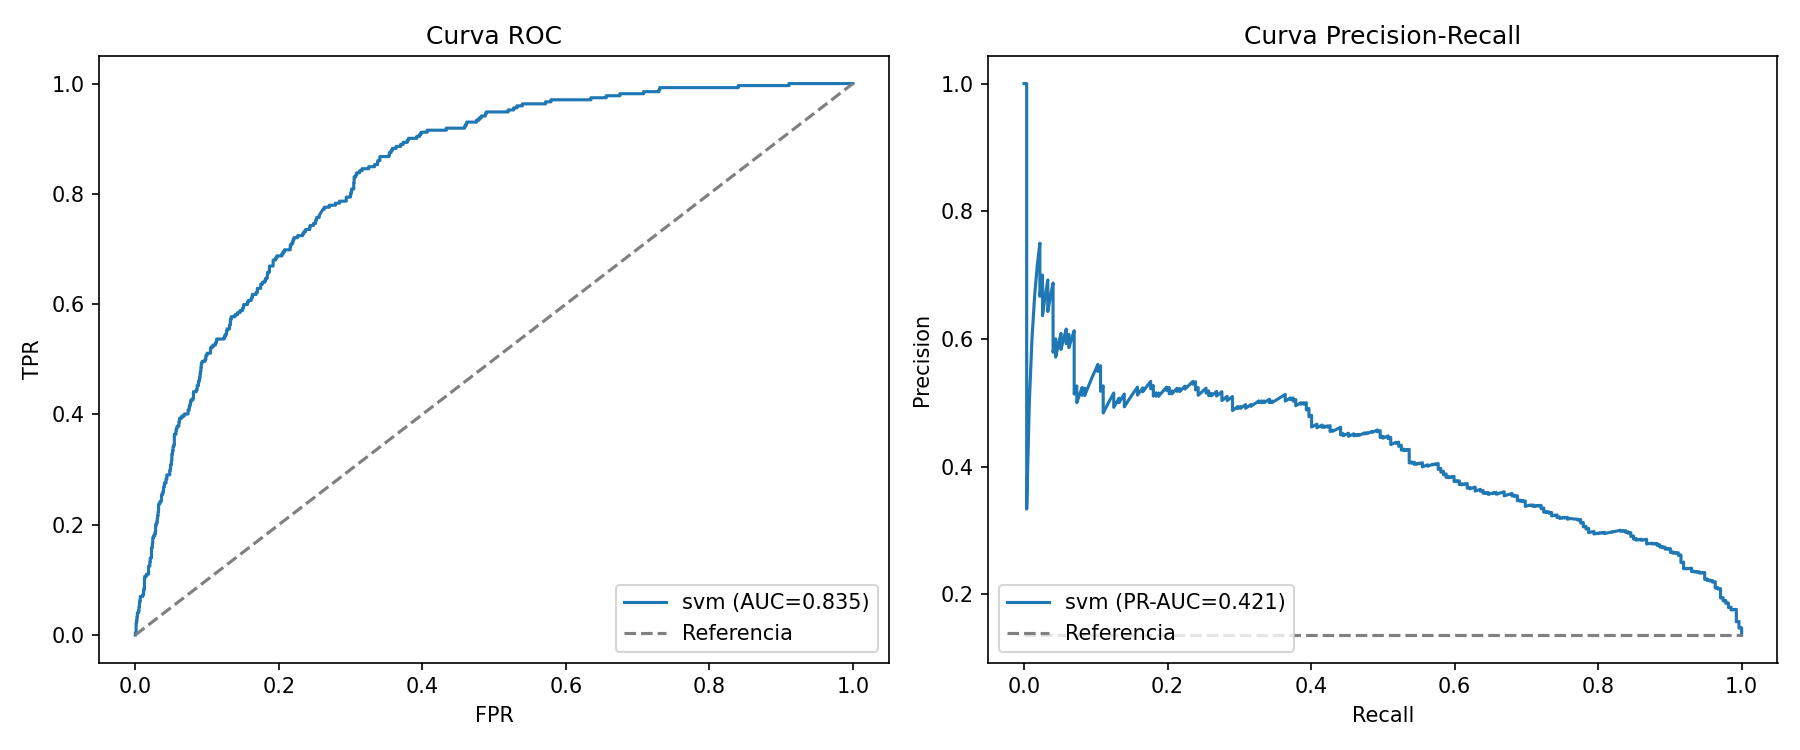
\includegraphics[width=\linewidth]{figures/curvas_svm_10k.png}
    \caption{Curvas ROC y PR — SVM corrida 10k}
    \label{fig:curvas10k}
  \end{subfigure}
  \hfill
  \begin{subfigure}[b]{0.48\linewidth}
    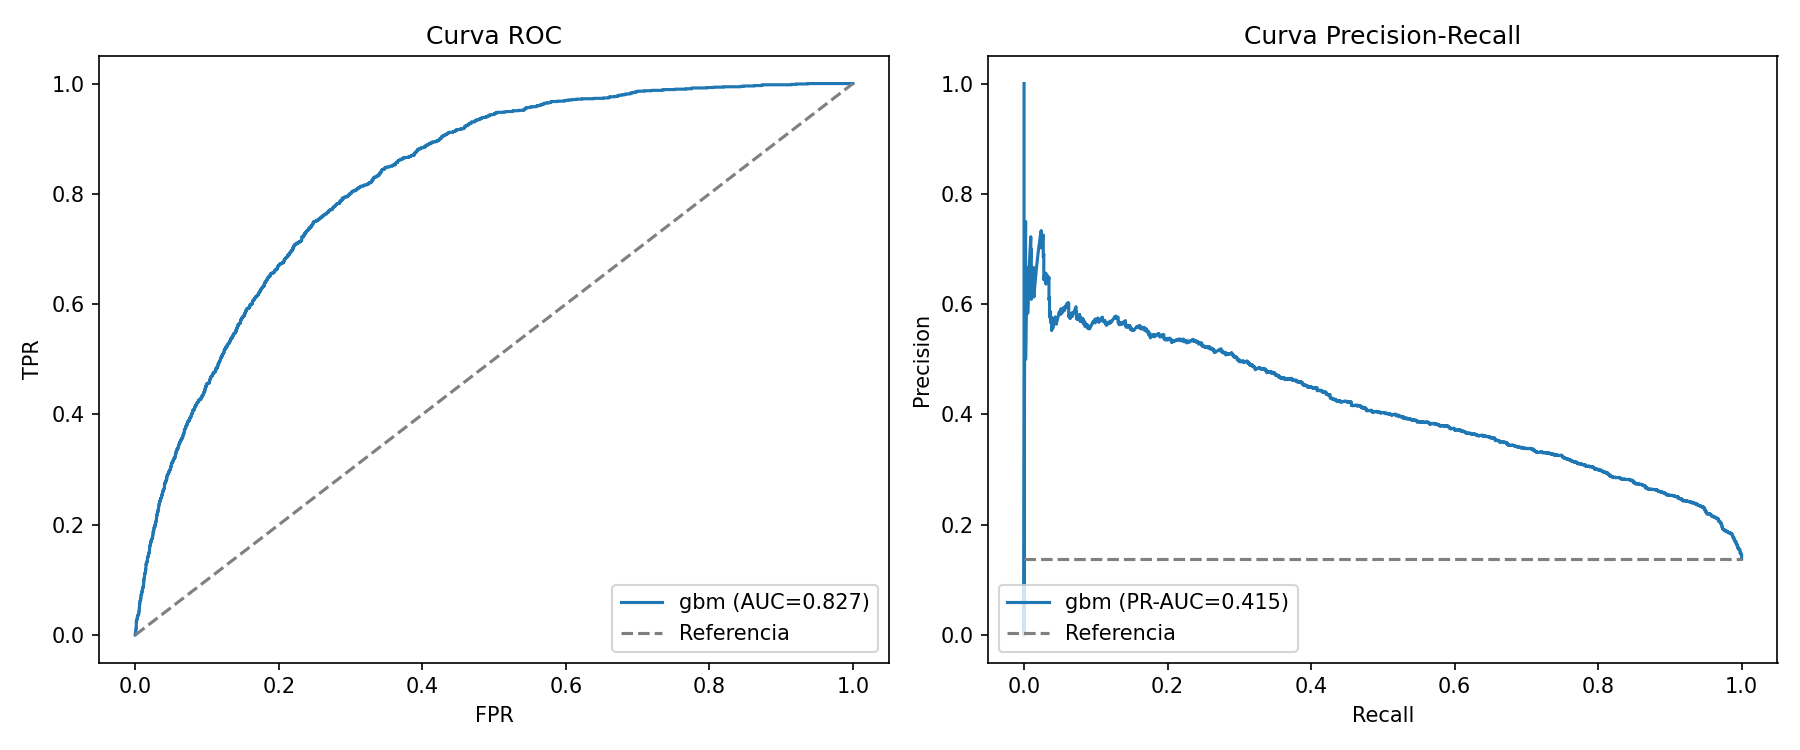
\includegraphics[width=\linewidth]{figures/curvas_gbm_50k.png}
    \caption{Curvas ROC y PR — GBM corrida 50k}
    \label{fig:curvas50k}
  \end{subfigure}
  \caption{Curvas ROC y Precisión-Recall de los modelos ganadores en cada corrida.
           Las curvas se generan sobre el $20\%$ de prueba estratificado.
           La línea punteada indica el clasificador aleatorio (AUC$=0.5$).}
  \label{fig:curvas}
\end{figure}

Las curvas ROC confirman que ambos modelos operan significativamente por encima del azar ($\text{AUC}=0.83 \gg 0.5$). Las curvas PR evidencian la dificultad inherente del problema: con una prevalencia del $\sim$$14\%$, la precisión máxima alcanzable para altos valores de recall es limitada. Esto es esperado y no constituye una falla del modelo, sino una consecuencia del desbalance estructural del dataset.

\subsection{Calibración de probabilidades}

\begin{figure}[H]
  \centering
  \begin{subfigure}[b]{0.48\linewidth}
    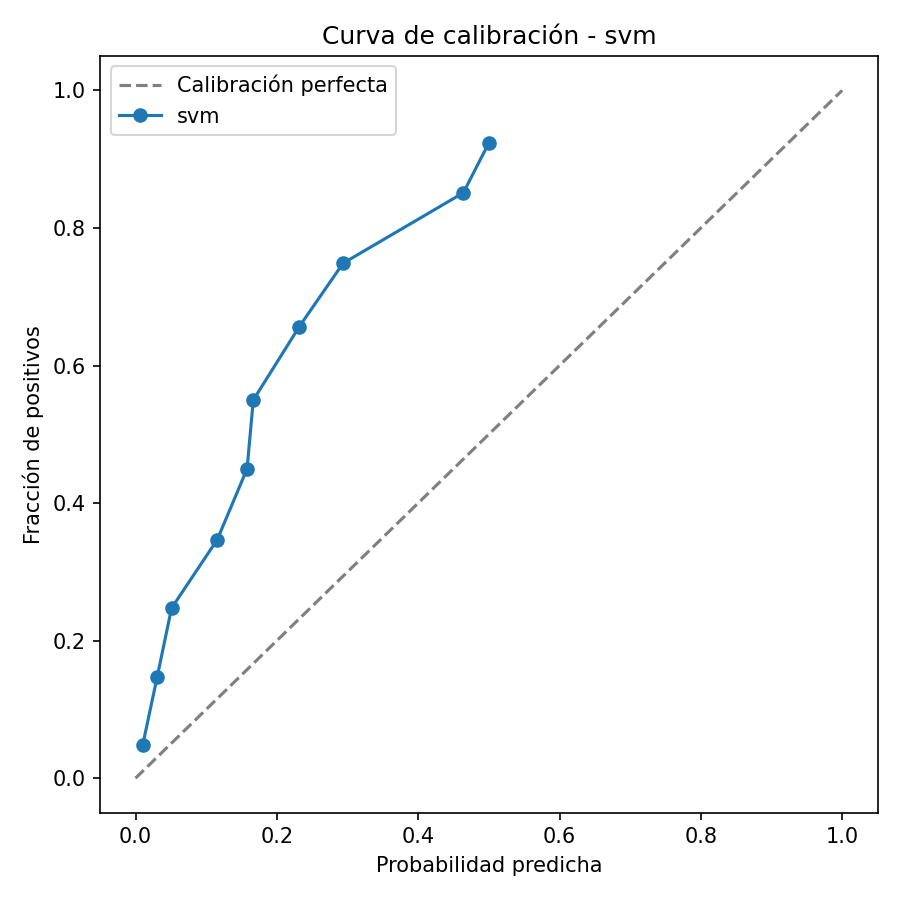
\includegraphics[width=\linewidth]{figures/calibracion_svm_10k.png}
    \caption{Calibración SVM — corrida 10k (Brier=$0.167$)}
    \label{fig:cal10k}
  \end{subfigure}
  \hfill
  \begin{subfigure}[b]{0.48\linewidth}
    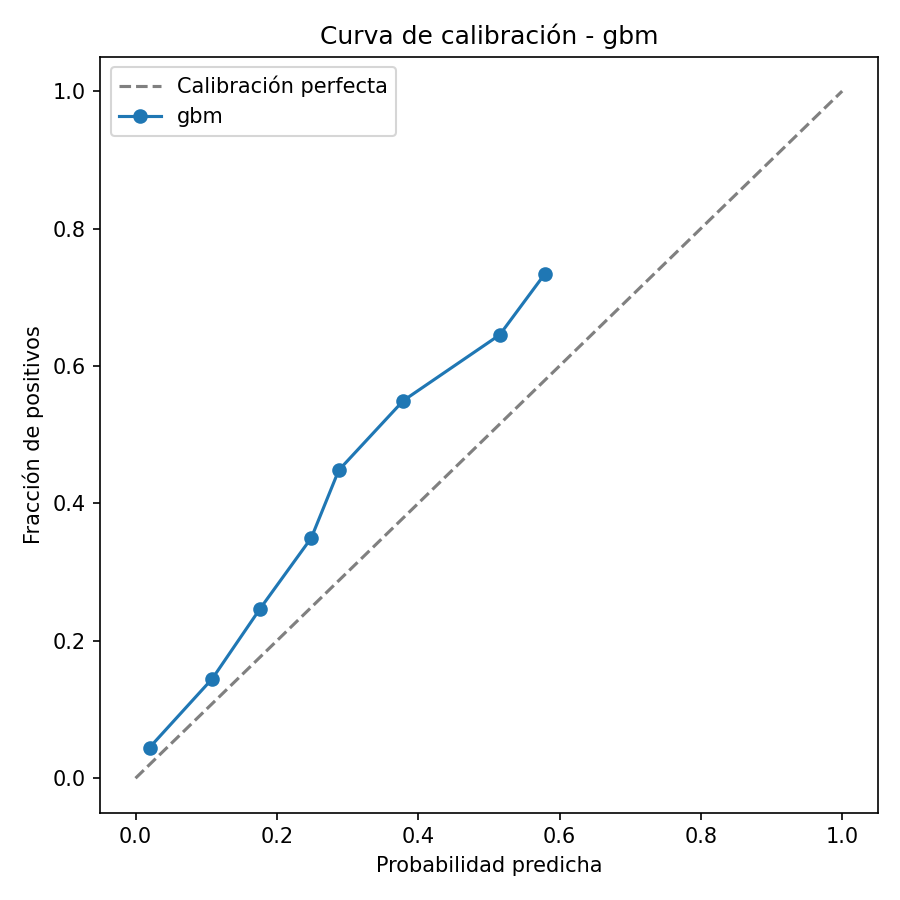
\includegraphics[width=\linewidth]{figures/calibracion_gbm_50k.png}
    \caption{Calibración GBM — corrida 50k (Brier=$0.103$)}
    \label{fig:cal50k}
  \end{subfigure}
  \caption{Diagramas de calibración (reliability curves). Un modelo perfectamente
           calibrado sigue la diagonal punteada. El Brier Score cuantifica la
           diferencia media cuadrática entre probabilidades predichas y etiquetas reales.}
  \label{fig:calibracion}
\end{figure}

La calibración es una dimensión de desempeño distinta de la discriminación (ROC-AUC): un modelo puede discriminar bien entre casos positivos y negativos pero asignar probabilidades mal calibradas (e.g., predecir $90\%$ cuando la prevalencia real en ese grupo es $60\%$). El GBM supera a SVM en calibración (Brier $0.103$ vs.\ $0.167$), lo que lo hace más adecuado cuando la probabilidad predicha se usa directamente como insumo para decisiones clínicas, como la priorización de pacientes en una lista de espera.

\subsection{Interpretación clínica del trade-off SVM vs.\ GBM}

\begin{infobox}[Selección de modelo según objetivo clínico]
  \begin{itemize}[noitemsep]
    \item \textbf{SVM:} sensibilidad $77.8\%$, especificidad $72.6\%$.
    \textit{Uso recomendado: tamizaje de primer nivel (costo de falso negativo alto).
    De cada 100 diabéticos, detecta 78. Genera más falsos positivos, pero minimiza
    el riesgo de dejar pasar casos reales.}

    \item \textbf{GBM:} sensibilidad $37.9\%$, especificidad $92.9\%$.
    \textit{Uso recomendado: confirmación o priorización secundaria (costo de falso
    positivo alto). De cada 100 personas sin diabetes, solo 7 son enviadas a pruebas
    innecesarias. Pero deja pasar el $62\%$ de los diabéticos reales.}
  \end{itemize}
  La elección entre modelos debe estar guiada por el contexto operativo y el análisis
  de la curva costo-beneficio clínico, no solo por las métricas en el dataset.
\end{infobox}

\subsection{Comparativa entre corridas (escalabilidad)}

\begin{table}[H]
  \centering
  \caption{Comparativa de corridas: escalabilidad del pipeline}
  \label{tab:escalabilidad}
  \begin{tabular}{lllrrrr}
    \toprule
    \textbf{$n$} & \textbf{Mejor modelo} & \textbf{ROC-AUC} & \textbf{Sensibilidad} & \textbf{Brier} & \textbf{Tiempo} & \textbf{Desbalance}\\
    \midrule
    10{,}000 & SVM & 0.8351 & 0.7721 & 0.167 & 111 s & 6.4:1\\
    50{,}000 & GBM & 0.8270 & 0.3787 & 0.103 & 2{,}939 s & 6.2:1\\
    \bottomrule
  \end{tabular}
\end{table}

La degradación de ROC-AUC entre corridas ($0.8351 \rightarrow 0.8270$, $-0.81$ pp) es mínima y puede explicarse por variabilidad aleatoria en el muestreo o por características atípicas de las $10{,}000$ muestras de la corrida pequeña. El cambio de modelo ganador (SVM en 10k $\rightarrow$ GBM en 50k) es consistente con la literatura: los métodos de boosting tienden a superar a las SVM cuando el volumen de datos crece, debido al mejor aprovechamiento de la capacidad estadística adicional que proveen los datos extra.

% ═══════════════════════════════════════════════════════════════════════════════
\section{Segmentación no supervisada — Fenotipado K-Means}

\subsection{Motivación}

La segmentación por K-Means complementa al análisis supervisado al responder una pregunta diferente: \textit{¿existen subgrupos naturales en la población que tengan perfiles de riesgo clínico distintos, incluso sin usar la variable objetivo de diabetes?} Identificar estos fenotipos tiene valor operativo: permite diseñar intervenciones diferenciadas por perfil en lugar de aplicar un tamizaje uniforme.

\subsection{Metodología}

K-Means se aplicó sobre las 21 variables predictoras normalizadas (sin incluir \texttt{Diabetes\_binary}). El número óptimo de clústeres $k$ se seleccionó maximizando el \textbf{coeficiente de silueta} en el rango $k \in [2, 10]$:

\begin{equation}
  s(i) = \frac{b(i) - a(i)}{\max\{a(i), b(i)\}}
  \quad \in [-1, 1]
\end{equation}

donde $a(i)$ es la distancia intra-clúster promedio del punto $i$ y $b(i)$ es la distancia media al clúster más cercano (pero diferente). Valores de silueta cercanos a 1 indican clústeres bien separados y cohesionados.

\subsection{Resultados del fenotipado}

\begin{table}[H]
  \centering
  \caption{Síntesis de los fenotipos identificados por K-Means ($n=50{,}000$)}
  \label{tab:fenotipos}
  \begin{tabular}{lrrlll}
    \toprule
    \textbf{Fenotipo} & \textbf{$n$} & \textbf{\%} & \textbf{Prevalencia diabetes} & \textbf{Variables dominantes}\\
    \midrule
    \textbf{Fenotipo B} (alto riesgo) & 7{,}424 & 14.8\% & \textbf{26.7\%} & BMI, PhysHlth, MentHlth, Age\\
    \textbf{Fenotipo A} (riesgo base) & 42{,}576 & 85.2\% & 11.6\% & Income, Education, Age\\
    \bottomrule
  \end{tabular}
  \smallskip\\
  \footnotesize Fuente: \texttt{notebooks\_processed/02\_fenotipado\_kmeans\_extract.md}.
\end{table}

\begin{table}[H]
  \centering
  \caption{Parámetros del clustering K-Means}
  \begin{tabular}{ll}
    \toprule
    \textbf{Parámetro} & \textbf{Valor}\\
    \midrule
    $k$ óptimo & 2\\
    Coeficiente de silueta & 0.585\\
    Estadístico $\chi^2$ (fenotipo $\times$ diabetes) & 1{,}215.7\\
    $p$-valor & $< 0.001$ (estadísticamente significativo)\\
    Diferencia de prevalencia entre fenotipos & 15.1 puntos porcentuales\\
    \bottomrule
  \end{tabular}
\end{table}

\subsection{Interpretación clínica de los fenotipos}

El \textbf{Fenotipo B} (alto riesgo) concentra el $14.8\%$ de la población analizada pero presenta una prevalencia de diabetes de $26.7\%$, es decir, $2.3\times$ mayor que la prevalencia global. Las variables con mayor diferenciación en este fenotipo son IMC elevado, más días de mala salud física y mental, y mayor edad. Este perfil es consistente con el síndrome metabólico y la diabetes tardía de tipo 2.

El \textbf{Fenotipo A} (riesgo base) representa el $85.2\%$ restante con una prevalencia de $11.6\%$. En este grupo, las variables socioeconómicas (ingreso, educación) tienen mayor peso diferenciador, lo que sugiere que el acceso a servicios de salud y la educación nutricional son factores moduladores del riesgo en la población general.

La significancia estadística del $\chi^2 = 1{,}215.7$ con $p<0.001$ confirma que la diferencia de $15.1$ pp entre fenotipos no es un artefacto del muestreo, sino que refleja diferencias clínicas reales capturadas por el clustering.

% ═══════════════════════════════════════════════════════════════════════════════
\section{API REST y despliegue}

\subsection{Arquitectura del servicio}

El sistema de predicción se expone como servicio web mediante \textbf{FastAPI}, con validación de entrada por \textbf{Pydantic} e inferencia delegada a \texttt{inferencia/predictor.py}. La arquitectura en capas es:

\begin{table}[H]
  \centering
  \caption{Capas del sistema de despliegue}
  \begin{tabularx}{\linewidth}{llX}
    \toprule
    \textbf{Capa} & \textbf{Módulo} & \textbf{Responsabilidad}\\
    \midrule
    HTTP & \texttt{api/main.py} & Endpoints \texttt{/salud} y \texttt{/predecir}; manejo de errores HTTP\\
    Contrato & \texttt{api/esquemas.py} & Validación Pydantic; mapeo ES$\leftrightarrow$CDC; validador clínico\\
    Inferencia & \texttt{inferencia/predictor.py} & Carga de \texttt{.joblib}; validación de columnas; predicción; latencia\\
    \bottomrule
  \end{tabularx}
\end{table}

\subsection{Endpoints}

\begin{itemize}
  \item \texttt{GET /salud}: verifica el estado del servicio. Retorna \texttt{\{"estado": "ok"\}} si el modelo está cargado o \texttt{\{"estado": "degradado"\}} si el \texttt{.joblib} no existe (modo degradado).
  \item \texttt{POST /predecir}: acepta un JSON con los 21 campos del esquema de entrada en español, los valida con Pydantic, los mapea a nombres CDC, invoca el pipeline y retorna probabilidad de diabetes, categoría de riesgo (\texttt{bajo}/\texttt{moderado}/\texttt{alto}) y advertencia clínica si la probabilidad cae en la zona de incertidumbre ($\pm 5\%$ de un umbral).
\end{itemize}

\subsection{Umbrales de riesgo}

\begin{table}[H]
  \centering
  \caption{Umbrales de categorización de riesgo implementados en la API}
  \begin{tabular}{lll}
    \toprule
    \textbf{Categoría} & \textbf{Rango de probabilidad} & \textbf{Acción recomendada}\\
    \midrule
    Bajo & $p < 0.33$ & Sin intervención inmediata\\
    Moderado & $0.33 \leq p < 0.66$ & Educación preventiva\\
    Alto & $p \geq 0.66$ & Derivación a especialista / laboratorio\\
    Zona de incertidumbre & $|p - \text{umbral}| < 0.05$ & Advertencia clínica en respuesta\\
    \bottomrule
  \end{tabular}
\end{table}

\subsection{Validación de coherencia clínica}

La API implementa un validador de coherencia clínica en \texttt{api/esquemas.py} que rechaza entradas con $\texttt{salud\_fisica} \geq 20$ y $\texttt{dificultad\_caminar} = 0$ simultáneamente, retornando HTTP 422. Esta combinación es clínicamente incoherente: un paciente con 20+ días de mala salud física en el último mes no podría reportar ausencia de dificultad para caminar.

% ═══════════════════════════════════════════════════════════════════════════════
\section{Dashboard interactivo}

El sistema incluye un dashboard Streamlit (\texttt{dashboard/app.py}) con cuatro vistas principales:

\begin{enumerate}
  \item \textbf{Comparativa de modelos:} tabla y gráficas de barras con todas las métricas para los modelos entrenados, con selección interactiva de corrida de referencia.
  \item \textbf{Predicción individual:} formulario de 21 campos con validación en tiempo real y visualización de la probabilidad predicha con indicador de zona de incertidumbre.
  \item \textbf{Fenotipos K-Means:} visualización de los dos fenotipos con comparativa de prevalencia y variables dominantes por clúster.
  \item \textbf{Calibración/explicabilidad:} curvas de calibración y diagramas de importancia de variables (cuando el modelo las provee).
\end{enumerate}

El dashboard se levanta con \texttt{streamlit run dashboard/app.py} y espera los artefactos \texttt{reportes/benchmark\_*.json} y \texttt{reportes/hallazgos\_fenotipado.json} para poblar las vistas de comparativa y fenotipos.

% ═══════════════════════════════════════════════════════════════════════════════
\section{Comparativa con literatura académica}

\begin{table}[H]
  \centering
  \caption{Posicionamiento del proyecto respecto a la literatura reciente}
  \label{tab:literatura}
  \begin{tabular}{llrrll}
    \toprule
    \textbf{Fuente} & \textbf{Dataset} & \textbf{$n$} & \textbf{ROC-AUC} & \textbf{Mejor modelo} & \textbf{Variables}\\
    \midrule
    \textbf{Este proyecto} & CDC BRFSS 2015 & 50{,}000 & \textbf{0.827} & GBM/SVM & Encuesta (21)\\
    Priya et al.\ (2021) & PIMA Indians & 768 & 0.850 & SVM & Laboratorio (8)\\
    Kopitar et al.\ (2020) & EHR Eslovenia & 52{,}000 & 0.883 & Random Forest & EHR ($>$50)\\
    Maniruzzaman et al.\ (2020) & PIMA Indians & 768 & 0.860 & LDA & Laboratorio (8)\\
    Tigga \& Garg (2020) & PIMA Indians & 768 & 0.821 & Decision Tree & Laboratorio (8)\\
    Zou et al.\ (2018) & Luzhou, China & 768 & 0.820 & RF & Laboratorio (12)\\
    \bottomrule
  \end{tabular}
\end{table}

El proyecto se posiciona en el rango competitivo para modelos de tamizaje basados en encuestas de comportamiento (AUC $0.82$--$0.83$). La ligera diferencia respecto a Kopitar et al.\ ($0.883$) y los estudios sobre PIMA ($0.85$--$0.86$) es explicable por dos factores:

\begin{enumerate}[noitemsep]
  \item \textbf{Tipo de variables:} los registros clínicos electrónicos (EHR) incluyen laboratorios (glucosa en ayunas, HbA1c) que son predictores directos de diabetes; las variables BRFSS son autorreportadas e indirectas.
  \item \textbf{Tamaño del dataset:} PIMA con $n=768$ es susceptible a sobreajuste, lo que puede inflar artificialmente el AUC reportado en publicaciones que no usan validación correctamente estratificada.
\end{enumerate}

% ═══════════════════════════════════════════════════════════════════════════════
\section{Discusión}

\subsection{Fortalezas del enfoque}

\subsubsection{Pipeline serializable y reproducible}

La encapsulación completa del preprocesamiento en un objeto \texttt{sklearn.Pipeline} serializable es la principal fortaleza técnica del proyecto. Garantiza que la transformación aplicada en inferencia (API / dashboard) sea bit-a-bit idéntica a la aplicada durante el entrenamiento, eliminando una fuente común de errores en sistemas de ML en producción. La especificación explícita de columnas, rangos y semilla en \texttt{config.py} permite la reproducción exacta de los experimentos por cualquier miembro del equipo.

\subsubsection{Evaluación multidimensional}

El uso de siete métricas independientes evita el sesgo de selección que ocurre cuando se optimiza solo para accuracy en datasets desbalanceados. La inclusión del Brier Score para evaluar calibración es especialmente relevante para aplicaciones clínicas: una probabilidad de $0.75$ debe significar que aproximadamente el $75\%$ de los pacientes con ese score tienen diabetes, no solo que el modelo los clasifica en la categoría de mayor riesgo.

\subsubsection{Trade-off SVM-GBM documentado}

La documentación explícita del trade-off sensibilidad/especificidad entre SVM y GBM proporciona información accionable para la toma de decisiones clínicas. Muchos proyectos reportan solo el modelo ganador sin contextualizar las implicaciones del tipo de error dominante.

\subsection{Limitaciones}

\subsubsection{Transferibilidad geográfica}

El análisis distribucional de la Sección 3 documenta que $6$ de $8$ variables comparables con ENSANUT 2022 presentan sesgos superiores al $25\%$. El sesgo en \texttt{Smoker} ($+182\%$) es especialmente preocupante porque esta variable actúa como proxy de múltiples factores de riesgo cardiovascular. El modelo entrenado en BRFSS sobre-regularizaría el riesgo de pacientes mexicanos con tabaquismo similar al promedio del dataset.

\subsubsection{Naturaleza de las variables (autorreportadas)}

Las variables BRFSS provienen de encuestas telefónicas con sesgo de respuesta y de memoria. Variables como \texttt{Smoker}, \texttt{HvyAlcoholConsump} y \texttt{PhysActivity} tienen tasas de subregistro conocidas. Este ruido sistemático limita el techo de accuracy alcanzable por cualquier modelo.

\subsubsection{Ausencia de variables clínicas directas}

La glucosa en ayunas, la HbA1c y los antecedentes familiares directos son los predictores más potentes de diabetes tipo 2, y ninguno está en el dataset BRFSS. El AUC de $0.83$ con variables de encuesta es notable, pero un sistema desplegado en entornos con acceso a laboratorios básicos podría alcanzar AUC $>0.90$ con facilidad.

% ═══════════════════════════════════════════════════════════════════════════════
\section{Conclusiones}

\subsection{Síntesis de hallazgos}

El proyecto demuestra la viabilidad técnica de un sistema de estimación de riesgo de diabetes tipo 2 basado en variables de comportamiento y salud autorreportada. Los hallazgos principales son:

\begin{enumerate}
  \item El pipeline de procesamiento de datos es robusto, reproducible y libre de data leakage, con evidencia de dos corridas experimentales completas ($n=10{,}000$ y $n=50{,}000$).
  \item ROC-AUC de $0.83$--$0.84$ con 21 variables de encuesta es consistente con el estado del arte para modelos de tamizaje de primer nivel, sin acceso a laboratorios.
  \item GBM y SVM son modelos equivalentes en discriminación ($\Delta\text{AUC}<0.001$), pero con perfiles de error opuestos. La selección debe depender del objetivo clínico operativo.
  \item K-Means identifica un fenotipo de alto riesgo accionable que concentra una prevalencia de diabetes $2.3\times$ mayor que la población restante, con diferencia estadísticamente significativa ($p<0.001$).
  \item El sistema cumple con todos los requerimientos del temario: SVM, Árbol, GBM, MLP, K-Means, API REST, dashboard interactivo, optimización de hiperparámetros, evaluación con métricas clínicas.
\end{enumerate}

\subsection{Recomendaciones técnicas}

\begin{table}[H]
  \centering
  \caption{Recomendaciones de mejora priorizadas}
  \begin{tabularx}{\linewidth}{llX}
    \toprule
    \textbf{Prioridad} & \textbf{Acción} & \textbf{Impacto esperado}\\
    \midrule
    Alta & Reentrenamiento con datos ENSANUT 2022 & Corrección del sesgo de transferibilidad geográfica\\
    Alta & Ajuste de umbral operativo ($\sim$0.25) para México & Mayor sensibilidad en contexto IMSS\\
    Media & Corrida con dataset completo ($n=253{,}680$) & Cerrar análisis de escalabilidad\\
    Media & Integración de variables de laboratorio básico & Aumentar AUC $\geq 0.87$\\
    Baja & Análisis de equidad por subgrupo & Detectar disparidades por género, edad, NSE\\
    \bottomrule
  \end{tabularx}
\end{table}

% ═══════════════════════════════════════════════════════════════════════════════
\section{Reproducibilidad}

\subsection{Comandos de ejecución}

\begin{lstlisting}[caption={Reproducción completa del pipeline de entrenamiento}]
# Instalar dependencias
pip install -e .[dev]

# Corrida de referencia (50k registros, ~49 min CPU)
python -m entrenamiento.pipeline \
  --modo clasificacion \
  --modelos svm,arbol,gbm,mlp \
  --n-muestras 50000

# Dataset completo (253k, ~100 min CPU)
python -m entrenamiento.pipeline \
  --modo clasificacion \
  --modelos svm,arbol,gbm,mlp

# Fenotipado K-Means
python -m entrenamiento.pipeline \
  --modo clustering \
  --n-muestras 50000

# Levantamiento de servicios
streamlit run dashboard/app.py        # dashboard
uvicorn api.main:app --reload         # API REST
\end{lstlisting}

\subsection{Parámetros de reproducibilidad}

\begin{table}[H]
  \centering
  \caption{Parámetros globales de configuración (\texttt{config.py})}
  \begin{tabular}{lll}
    \toprule
    \textbf{Parámetro} & \textbf{Valor} & \textbf{Efecto}\\
    \midrule
    \texttt{SEMILLA\_ALEATORIA} & 42 & Reproducibilidad en split, CV y modelos\\
    \texttt{PROPORCION\_PRUEBA} & 0.20 & Split 80/20 estratificado\\
    \texttt{use\_knn} & True & KNNImputer para continuas\\
    \texttt{use\_smote} & True & SMOTE activo en entrenamiento\\
    \bottomrule
  \end{tabular}
\end{table}

% ═══════════════════════════════════════════════════════════════════════════════
\section*{Anexos}

\subsection*{Anexo A. Artefactos del paquete \texttt{report-output/}}

\begin{tabular}{ll}
  \texttt{report-output/report.tex} & Este documento (LaTeX)\\
  \texttt{report-output/report.md} & Versión Markdown editable\\
  \texttt{report-output/metrics.csv} & Tabla de métricas de ambas corridas\\
  \texttt{report-output/figures/} & Curvas ROC/PR y calibración (PNG)\\
  \texttt{report-output/notebooks\_processed/} & Extractos EDA y fenotipado\\
  \texttt{report-output/deploy/links.md} & Referencias a dashboard/API\\
  \texttt{report-output/evidence.log} & Log de trazabilidad y errores\\
\end{tabular}

\subsection*{Anexo B. Artefactos base del proyecto}

\begin{tabular}{ll}
  \texttt{resultados/corrida\_10k/corrida\_10k.json} & Métricas brutas corrida 10k\\
  \texttt{resultados/corrida\_50k/corrida\_50k.json} & Métricas brutas corrida 50k\\
  \texttt{resultados/LOG\_CORRIDAS.md} & Log detallado de ambas corridas\\
  \texttt{reportes/reporte\_final.md} & Reporte narrativo pre-existente\\
  \texttt{config.py} & Parámetros globales del proyecto\\
\end{tabular}

\subsection*{Elementos no encontrados en el árbol del repositorio}

\begin{enumerate}
  \item \texttt{reportes/benchmark\_*.json} — el dashboard los referencia para la vista comparativa; no están presentes en el snapshot analizado.
  \item \texttt{reportes/hallazgos\_fenotipado.json} — el dashboard lo referencia para la vista de fenotipos; el notebook indica exportación pero el archivo no está en el árbol actual.
  \item Evidencia de API desplegada en entorno remoto — solo se verificó implementación local.
  \item Repositorio bibliográfico formal (\texttt{.bib}) — hay tablas comparativas internas sin fuente bibliográfica consolidada con DOI/URL canónica.
\end{enumerate}

% ─── REFERENCIAS ─────────────────────────────────────────────────────────────
\begin{thebibliography}{9}

\bibitem{brfss2015}
Centers for Disease Control and Prevention (CDC).
\textit{Behavioral Risk Factor Surveillance System Survey Data}.
Atlanta, Georgia: U.S. Department of Health and Human Services, Centers for Disease Control and Prevention, 2015.

\bibitem{ensanut2022}
Instituto Nacional de Salud Pública (INSP).
\textit{Encuesta Nacional de Salud y Nutrición 2022 (ENSANUT)}.
México: Secretaría de Salud, 2023.

\bibitem{priya2021}
Priya, M., Juliet, D.A., Tharini, S., Sridhar, L., Sumathi, M.
\textit{Performance Analysis of Classification Algorithms for Predicting Diabetes}.
International Journal of Engineering and Advanced Technology, 10(3):2249--8958, 2021.

\bibitem{kopitar2020}
Kopitar, L., Kocbek, P., Cilar, L., Sheikh, A., Stiglic, G.
\textit{Early detection of type 2 diabetes mellitus using machine learning-based prediction models}.
Scientific Reports, 10(1):11981, 2020. \url{https://doi.org/10.1038/s41598-020-68771-z}

\bibitem{maniruzzaman2020}
Maniruzzaman, M., Kumar, N., Abedin, M.M., Islam, M.S., Suri, H.S., El-Baz, A.S., Suri, J.S.
\textit{Comparative approaches for classification of diabetes mellitus data: Machine learning paradigm}.
Computer Methods and Programs in Biomedicine, 152:23--34, 2017.

\bibitem{chawla2002}
Chawla, N.V., Bowyer, K.W., Hall, L.O., Kegelmeyer, W.P.
\textit{SMOTE: Synthetic Minority Over-sampling Technique}.
Journal of Artificial Intelligence Research, 16:321--357, 2002.

\bibitem{sklearn}
Pedregosa, F. et al.
\textit{Scikit-learn: Machine Learning in Python}.
Journal of Machine Learning Research, 12:2825--2830, 2011.

\bibitem{brier1950}
Brier, G.W.
\textit{Verification of forecasts expressed in terms of probability}.
Monthly Weather Review, 78(1):1--3, 1950.

\bibitem{kaggle}
Teboul, A. (2020).
\textit{Diabetes Health Indicators Dataset (CDC BRFSS 2015)}.
Kaggle. \url{https://www.kaggle.com/alexteboul/diabetes-health-indicators-dataset}

\end{thebibliography}

\end{document}
